\documentclass[a4paper,10pt]{article}
\usepackage[utf8x]{inputenc}
\usepackage{dirtree}
\usepackage[margin=1in]{geometry}
\usepackage[UKenglish]{babel}
\usepackage[fixlanguage]{babelbib}
\usepackage[square,sort,nonamebreak,comma]{natbib}  % citação bibliográfica alpha (alpha-ime.bst)
\usepackage{listings}
\usepackage{amsmath}
\usepackage{amsfonts}
\usepackage{amssymb}
\usepackage{graphicx}
\usepackage{hyperref}


\title{iModel: Icosahedral grid tools for geosphysical fluid dynamics modelling}
\author{Pedro S. Peixoto (pedrosp@ime.usp.br)}

\begin{document}
\maketitle

The software is a pack of tools to work with icosahedral and Voronoi geodesic grid based geophysical fluid models. It contains
\begin{itemize}
 \item Grid generator and grid tools, including grid optimization
 \item Interpolation and vector reconstruction pack
  \item A Multigrid solver
 \item A transport model
 \item A shallow water model 
\end{itemize}



This code is mainly for research and educational purposes. It is in constant change and has not been tested for all its configurations possibilities. 

    This program is free software: you can redistribute it and/or modify
    it under the terms of the GNU General Public License as published by
    the Free Software Foundation.

    This program is distributed in the hope that it will be useful,
    but WITHOUT ANY WARRANTY. See the GNU General Public License for more details.


For references check my website: \url{www.ime.usp.br/~pedrosp}. Do not hesitate to contact me in case of problems or doubts. Please contact me if you wish to have pre-calculated optimized grids, since they are very large, they are not shipped with the code.


\section{Requirements}

The software is very much self contained and does not rely on extra third party software other than the compiler. It is built for \textbf{linux platforms}, but may be run on Windows via Cygwin.

It was designed to run with very basic Fortran 90 coding, therefore tends to runs on any version of \textbf{GNU gfortran} compilers or \textbf{Intel ifort} compilers. Intel compiler will chosen as default if installed.

The outputs of the program are either text files or maps with binary data files. The maps are outputted to be read and graphed using \textbf{Generic Mapping Tool} (Version 4.x.x), and several scripts for this purpose are provided.

Some output data can be easily analysed in Matlab, but since they are outputted as text files, any other software may be used.

The code is not very optimized, but uses openmp shared memory parallelism in many places.

\section{Code structure}

Main files of program

\dirtree{%
.1 imodel/ \hspace{1cm}  \begin{minipage}[t]{10cm}
                  Makefile \\
		  readme{.}txt\\
                \end{minipage}.
.2 bin/ \hspace{1cm}  \begin{minipage}[t]{10cm}
          This directory holds executable files (binary files)\\
          \end{minipage}.
.2 data/ \hspace{1cm}  \begin{minipage}[t]{10cm}
          Directory where output from imodel is written\\
          \end{minipage}.
.2 doc/ \hspace{1cm}  \begin{minipage}[t]{10cm}
          Directory for documentation\\
          \end{minipage}.
.2 gmt/ \hspace{1cm}  \begin{minipage}[t]{10cm}
          Generic Mapping Tool (GMT) scripts\\
          \end{minipage}.
.3 {.}sh \hspace{1cm}  \begin{minipage}[t]{10cm}
          GMT bash scripts\\
	  the main one being plot{.}sh for plotting grids, scalar and vector fields\\
	  anin{.}sh may be used to create animations\\
	  \end{minipage}.
.3 {.cpt} \hspace{1cm}  \begin{minipage}[t]{10cm}
	    Color pallets \\
          \end{minipage}.
.2 graphs/ \hspace{1cm}  \begin{minipage}[t]{10cm}
          Output directory for GMT maps (eps and pdf)\\
          \end{minipage}.
.2 grid/ \hspace{1cm}  \begin{minipage}[t]{10cm}
          Directory for all grid files\\
	  iModel will automatic save and load the grids from this directory\\
	  GMT will read grid files from this directory to draw figures of grids\\
          \end{minipage}.
.3 {.}dat \hspace{1cm}  \begin{minipage}[t]{10cm}
          Fortran binary files with saved grid information to be loaded\\
	  \end{minipage}.
.3 {.gmt} \hspace{1cm}  \begin{minipage}[t]{10cm}
	    Text grid files for GMT to read and graph\\
          \end{minipage}.
.2 matlab/ \hspace{1cm}  \begin{minipage}[t]{10cm}
          Directory for matlab scripts\\
          \end{minipage}.
.2 par/ \hspace{1cm}  \begin{minipage}[t]{10cm}
          Directory for input parameter files
          \end{minipage}.
.3 mesh{.}par \hspace{1cm}  \begin{minipage}[t]{10cm}
          Parameters for grid to be used (generate or load)\\
	  \end{minipage}.
.3 simul{.}par \hspace{1cm}  \begin{minipage}[t]{10cm}
	    Parameters for several simulations of differential operator and interpolation testing\\
          \end{minipage}.
.3 multigrid{.}par \hspace{1cm}  \begin{minipage}[t]{10cm}
	    Parameters for Multigrid solver\\
          \end{minipage}.
.3 trans{.}par \hspace{1cm}  \begin{minipage}[t]{10cm}
	    Parameters for Semi-Lagrangian Transport model\\
          \end{minipage}.
.3 swm{.}par \hspace{1cm}  \begin{minipage}[t]{10cm}
	    Parameters for Shallow Water Model\\
          \end{minipage}.
.2 ref/ \hspace{1cm}  \begin{minipage}[t]{10cm}
          Directory for reference solutions\\
	  Currently has ENDGame source files\\
	  Reference solutions will be read from this directory\\
	  Edit eg-swm-ref-{.}f90 and run Makefile to create the reference data \\
	  See EG-refsoln-doc{.}pdf for details
          \end{minipage}.
.2 sh/ \hspace{1cm}  \begin{minipage}[t]{10cm}
          Bash scripts to run several instances of the program with different parameter configurations
          \end{minipage}.
.2 src/ \hspace{1cm}  \begin{minipage}[t]{10cm}
          Fortran 90 source files and extra bash scripts\\
          \end{minipage}.
.3 imodel{.}f90 \hspace{1cm}  \begin{minipage}[t]{10cm}
          Main driver for program\\
	  Use par/mesh{.}par to select which program component you want to run\\
	  \end{minipage}.
.3 constants{.}f90 \hspace{1cm}  \begin{minipage}[t]{10cm}
          Refers to all constants used in the program\\
	  \end{minipage}.
.3 datastruct*{.}f90 \hspace{1cm}  \begin{minipage}[t]{10cm}
          Refers to all datastructure used for the grids\\
	  datastruct{.}f90 is general and datastructmult{.}f90 is for the multigrid solver \\
	  \end{minipage}.
.3 stripackm{.}f90 \hspace{1cm}  \begin{minipage}[t]{10cm}
	    Robert Renka Algorithm 772 for Parameters for Delaunay Triangulation and Voronoi Diagram on the Surface of a Sphere\\
          \end{minipage}.
.3 smeshpack{.}f90 \hspace{1cm}  \begin{minipage}[t]{10cm}
          Main program for grid generation \\
	  Has many tools to load and work with geodesic grids\\
	  Configure it using par/mesh{.}par
	  \end{minipage}.
.3 interpack{.}f90 \hspace{1cm}  \begin{minipage}[t]{10cm}
          Pack with scalar and vector interpolation routines \\
	  \end{minipage}.
.3 diffoperpack{.}f90 \hspace{1cm}  \begin{minipage}[t]{10cm}
          Pack with some discrete differential operators\\
	  \end{minipage}.
.3 simulpack{.}f90 \hspace{1cm}  \begin{minipage}[t]{10cm}
          Main program for simulations with interpolations and basic discrete differential operator analysis\\
	  Parameters set with par/simul{.}par\\
	  \end{minipage}.
.3 multigrid{.}f90 \hspace{1cm}  \begin{minipage}[t]{10cm}
	    Multigrid solver\\
          \end{minipage}.
.3 transport{.}f90 \hspace{1cm}  \begin{minipage}[t]{10cm}
	    Semi-Lagrangian transport model\\
          \end{minipage}.
.3 swm{.}f90 \hspace{1cm}  \begin{minipage}[t]{10cm}
	    Shallow Water Model\\
	    Relies on data structure dataswm{.}f90
	    \end{minipage}.
.4 dataswm{.}f90 \hspace{1cm}  \begin{minipage}[t]{10cm}
	    Shallow Water Model data structure\\
          \end{minipage}.
.3 *{.}sh \hspace{1cm}  \begin{minipage}[t]{10cm}
	    Scripts for: \\
	    Code archive to tar.bz2 (tarfiles)\\
	    Code backup (backup)\\
	    Verify compiler (compiler) \\
	    Create program directory structure (dirs) \\
	    Create binary link for imodel (link) \\
          \end{minipage}.
}
 
\section{Usage and Pre-setup programs}

Type ``make'' to compile all source code. Use the parameter files in ``par/*.par'' to setup what you wish to run. Run with ``./imodel'' from the main folder.

Programs already setup. Select in par/mesh.par:\\
\begin{verse}
!  case(1) !Test geodesic to regular grid conversion tool\\
!  case(2) !Test grid point search methods\\
!  case(3) !Mesh quality and distortion tests\\
!  case(4) !Divergence Tests\\
!  case(5) !Laplacian Tests\\
!  case(6) !Test scalar interpolations\\
!  case(7) !Test vector interpolation\\
!  case(8) !Test vector reconstruction\\
!  case(9) !Passive advection simulation\\
!  case(10)!Transport flow simulation\\
!  case(11)!Multigrid tests\\
!  case(12)!Tg reconstruction test\\
!  case(13)!Rotational discretization test\\
!  case(14)!Horizontal Discret Shallow water model diagnostics\\
!  case(15)!Shallow water model test cases\\
\end{verse}


\section{Grid generator}

The grid generator creates spherical triangular grids with its dual Voronoi grid and all the necessary relationship between nodes, edges, triangles and Voronoi cells (see datastruct.f90 for details). All the grid specifications need to be setup um par/mesh.par.

Kinds of grids generated:\\
\begin{verse}
!   icos (icosahedral) \\
!   octg (octahedral) \\
!   read (read from file - give filename where indicated) \\
!   rand (random points - be careful, you can get ugly meshes...) \\
\end{verse}

When using `icos' or `octg', you need to specify the number of nodes wanted as well. It does not need to be exact, as the code will adjust the next icosahedral or octahedral grid with the proper number of nodes.

You may read grid nodes from a text file. This may be with lat/lon  coordinates (which should have extension .gmt) or x/y/z coordinates (which should have extension .xyz) of the points. For x/y/z coordinates, you must first add the number of nodes that will be read. For lat/long, this is not necessary. The order of the points may matter, as we do not want to have the first 3 points aligned. A file with the connection from one node to its neighbour indexes may also be read with extension .ngb (the mesh generator will check if the ngb file exists, if so, use it). These files must be in the grid/ folder in runtime.

The position of the mesh with respect to geographic coordinates may be chosen from:\\
!Mesh Positions \\
\begin{verse}
!  eqs (equator symmetric)\\
!  pol (north pole point)\\
!  ran (all random points)\\
!  ref (local mesh refinement - needs scvt optimization)\\
\end{verse}

Once the grid is generated, you may use all the pre computed data stored in the datastruct of type `mesh'. You may chose to save the generated grid to later load it directly from the binary files.

A regular latitude-longitude grid table containing for each latitude-longitude box the index of the grid nodes it intersects is also generated. This allows a very quick search within the grid, since the regular grid resolution is calculated to be very fine and have on average almost only 1 grid cell intersection. This is useful in Semi-Lagrangian methods, or other procedures that require interpolations of arbitrary points. 

\subsection{Grid optimizations}

The grid generator has the following grid optimizers coded:\\
!Optimization of mesh \\
\begin{verse}
!  nopt (no optimization) \\
!  sprg (spring dynamics - ok until level 8) \\
!  scvt (centroidal voronoi) \\
!  salt (aligned tesselation - not debuged ...) \\
!  hr95 (Heikes and Randall 1995 optimization using Miura's alg - not debuged...) \\
\end{verse}

The `salt' optimization tries to align a grid with respect to the index given in \cite{Peixoto2013}, but is not successful. The HR95 grid optimizer is not producing the expected results. It uses and algorithm proposed by  \cite{Miura2005}, that does not seem to converge properly. 

There is an option to generate locally refined grids with SCVT tessellations, as in \cite{Ringler2013}. The density function needs to be set in src/smeshpack.f90 function dens\_f. Also, option regarding the way the grid is constructed, recursively (hierarchically)or not.\\

!Hierarchical grid construction: \\
!  0-No; \\
!  1-Yes; \\
!  2 - Optimizes only the new points in hierarchy; \\
!  3 - Do not optimize nodes that belong to primary icosahedral edges\\

\subsection{Testing}
The main testing programs can be selected in the par/mesh.par file as one of the bellow.\\
!  case(1) !Test geodesic to regular grid conversion tool\\
!  case(2) !Test grid point search methods\\
!  case(3) !Mesh quality and distortion tests\\


\subsection{Grid visualization and examples}

To view the grid generated, go to the gmt/ folder and use the `plot.sh' script. You need to provide as command line input the name of the grid you want to be plotted. This is done by passing the name of the file that contain the `*nodes.gmt' in the grd/ folder. The script will guide you through its options, for either plotting just the triangular grid, Voronoi grid and other options. Outputs will be placed in graphs/ folder. Edit plot.sh to fulfil your needs.

\subsubsection{Example 1 - icosahedral grid level 2}
To generate the grid set in par/mesh.par the following parameters (leave the rest as default):
No. of vertices: 42 \\
Kind of mesh: icos \\
Optimization: nopt \\
Run any program of grid testing, e.g. cases 1,2,3, or actually any other test case should generate the grid.
\begin{lstlisting}[language=bash]
$ ./imodel
\end{lstlisting}
Once the grid is generated, run:
\begin{lstlisting}[language=bash]
$ cd gmt
$ ./plot.sh ../grid/icos_pol_nopt_2_nodes.gmt 
Options : 1-> 1-> 6
Output in graphs/icos_pol_nopt_2.pdf
\end{lstlisting}

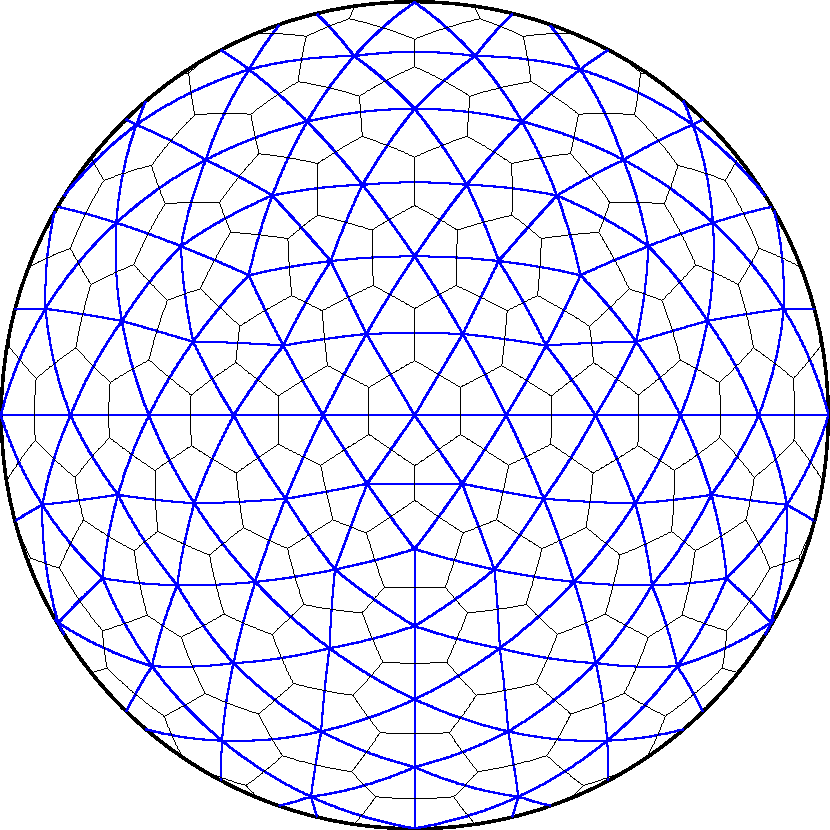
\includegraphics[scale=0.5]{icos_pol_nopt_2}

\subsubsection{Example 2 - Locally refined grid}

Follow the same example as above, but set grid parameters in par/mesh.par to:
No. of vertices: 600 \\
Kind of mesh: icos \\
Position: ref \\
Optimization: scvt \\
It will start from icosahedral grids and use SCVT algorithms to get locally refined ones based on a density function given in src/smeshpack.f90 function dens\_f. The generation can take some minutes.

\begin{lstlisting}[language=bash]
$ cd gmt
$ ./plot.sh ../grid/icos_ref_scvt_h1_3_nodes.gmt 
Options : 1-> 1-> 5
Output in graphs/icos_ref_scvt_h1_3.pdf
\end{lstlisting}

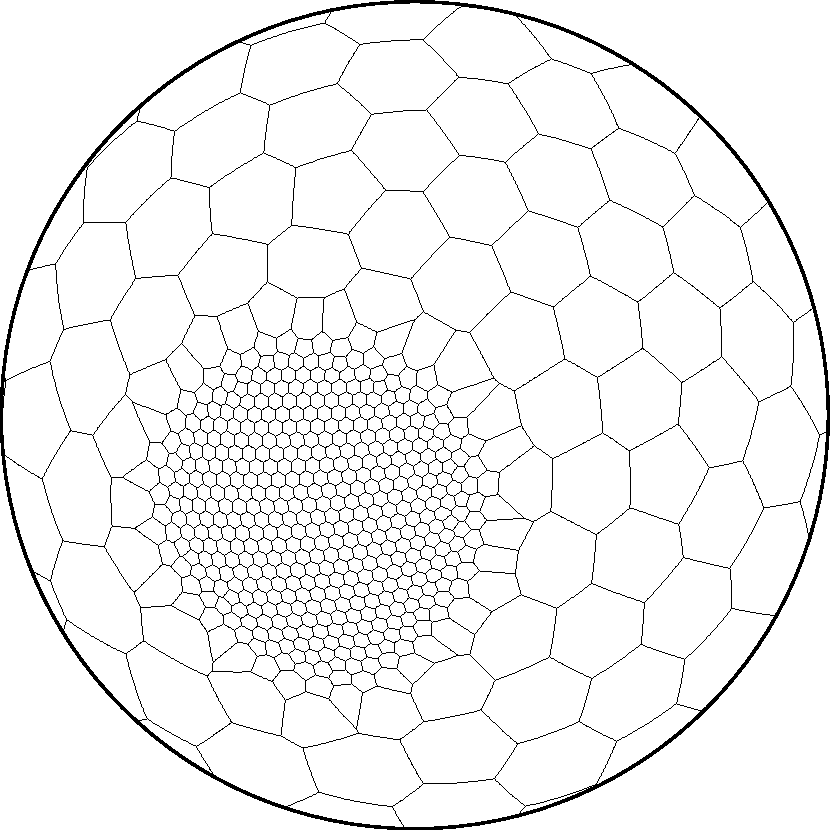
\includegraphics[scale=0.5]{icos_ref_scvt_h1_3}

\subsection{Important}

Some grid generations with optimizations can take hours and even days (months in case of very fine grids). The grid points are saved in .xyz of .gmt for future use in this or other codes. All the grid structures and pre calculated features are store as well, and this can be loaded at runtime setting the load option in par/mesh.par. Setting the read option in par/mesh.par read only the node points in cartesian or lat-long coordinates, but regenerates all other data structures and pre computable mesh properties. Please contact me if you wish to have pre-calculated optimized grids, since they are very large, they are not shipped with the code.


\section{Interpolations}

The main module for interpolations on spherical geodesic grids is src/interpack.f90. It contains several kinds of methods and possibilities. These maybe set via par/simul.par, and several testing programs exist to analyse the methods.

\subsection{Variable location}

The variables may be located in the grid in the following different ways:\\
  ! List of Stags for interpolation - (if no vector - considers scalars on vector positions)\\
  ! HA  - Scalars and vectors on triangle vertices, hexagon centers\\
  ! HC  - Scalars on triangle vertices, hexagon centers and vectors hexagon edge midpoints\\
  ! TA  - Scalars and vectors on triangle circumcenter, hexagon vertices\\
  ! TC  - Scalars on triangle vertices, hexagon centers and vectors triangle edge midpoints\\
  ! HCT - Voronoi staggered grid but with vectors on intersection of hx edge and tr edge.\\
 
Note: Not all methods are implemented for all positionings.

\subsection{Scalar interpolations}

Implemented scalar interpolation methods:\\
    !*** (For values given on triangle vertices - Stag=HA) ***\\
    ! none     = Just get triangle\\
    ! neartrv  = Nearest node  (default)\\
    ! lintrv   = Linear TR - values on tr vertices - default\\
    ! linhxb   = Linear TR - values on Voronoi cell centroids\\
    ! lsqhx    = Quadratic Least Squares \\
    ! hermtrv  = Cubic (R.Renka C1 Hermite)\\
    ! rbftr    = RadialBasisFunction TR (3pts)\\
    ! rbfetr   = RadialBasisFunction ETR(11,12pts)\\
    ! rbfhx    = RadialBasisFunction HX (6,7pts)\\
    ! natlap   = Natural Coordinate with Laplace\\
    ! natsib   = Natural Coordinate with Sibson\\
    ! natfar   = Natural Coordinate with Farin\\
    ! lmshep   = Local Modified Shepard Method\\
    ! qdshep   = Quadratic Shepard Method\\
    !*** (For values given on triangle circumcenters - Stag=TA) ***\\
    ! none     = Just get triangle\\
    ! neartrc  = Nearest triangle\\
    ! wach     = Wachspress interpolation - default\\
    !*** (For values given on triangle edge midpoints - Stag=TC) ***
    ! none     = Just get triangle\\
    ! p1nc     = P1 Non corforming element - default\\
    !*** (For values given on voronoi edge midpoints - Stag=HC) ***
    ! none     = Just get triangle \\
    ! wach     = Modified Wachspress interpolation (linear) - default \\
    ! lmshep   = Local Modified Shepard Method\\
    ! p1nc     = P1 Non corforming element - may do extrapolation\\
    !*** (For values given on Voronoi centroids) ***\\
    ! neartrv  = Nearest node  (default)\\
    !*** (For values given on triangle centroids) ***\\
    ! neartrc  = Nearest triangle  (default)\\


    Use "none" to set no interpolation. Used only to calculate basic computational cost. Some of these scalar interpolations, such as `lintrv' and `wach', may be used to do vector interpolation when the full vector is given pointwise.

\subsection{Vector reconstructions}

See \cite{Peixoto2014} for the vector reconstruction problem definition and methods. The methods implemented are as follows.

    !Kind of reconstruction\\
    !  none   = Just find the nearest node\\
    !  rbf    = Radial Basis Function\\
    !     rbfhx  - rbf for 6 point Voronoi cell\\
    !     rbftr  - rbf for 3 point triangle\\
    !     rbf*pc- rbf* with constant polynomial\\
    !  per    = Perot (2000) recosntruction\\
    !     perhx  - Perot for Hexagons\\
    !     pertr  - Perot for Triangles\\
    !     perpj  - Perot for Hexagons projecting to tang plane\\
    !     pered  - Perot vector for edges (tangent recon)\\
    !  lsq    = Least Square Fit\\
    !     lsqhxe - 12 point hexagon stencil\\
    !     lsqtrc - 9 point triangle based stencil\\
    !  rt0    = Raviart Thomas 0th order element reconstruction\\
    !  dtred  = Dual triangle tangent reconstruction\\
    !  wht    = Whitney Edge element reconstruction\\
    !  kls    = Klausen reconstruction with Wachspress coords\\
    !  trsk   = TRISK tangent vector reconstruction\\

\subsection{Testing}
The main testing programs can be found in src/simulpack.f90, and the test can be selected in the par/mesh.par file as one of the bellow.\\
!  case(6) !Test scalar interpolations\\
!  case(7) !Test vector interpolation\\
!  case(8) !Test vector reconstruction\\
!  case(12)!Tg reconstruction test\\

There are several scalar and vector function options that can be selected, see par/simul.par.

Once a test has been run, the results are stored in data/ folder with either numerical text files (for errors and diagnostics) or .dat files, for field plots. To plot a field, you can use the plot.sh GMT script. 

Example setting staggering to HA in par/simul.par and keeping the rest default - shows the exact scalar function to be interpolated:
\begin{lstlisting}[language=bash]
$ cd gmt
$ ./plot.sh ../data/sinterp_f5_HA_lintrv_exact_icos_pol_nopt_5.dat 
Options : 2-> 2-> 0-> 6
Output in ../graphs/sinterp_f5_HA_lintrv_exact_icos_pol_nopt_5.pdf
\end{lstlisting}
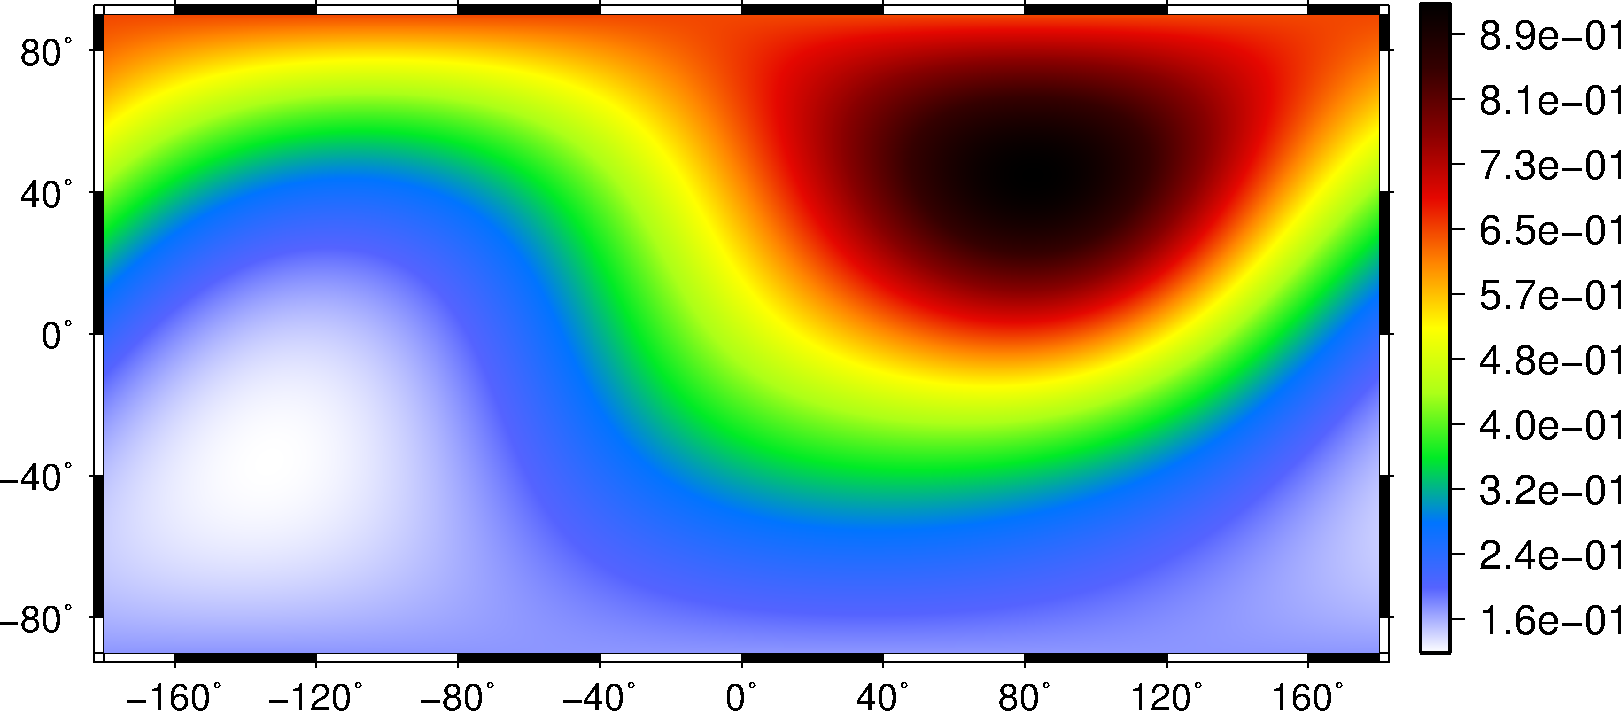
\includegraphics[scale=0.5]{sinterp_f5_HA_lintrv_exact_icos_pol_nopt_5}


\section{Differential operators}

The analysis of the differential operator done in \cite{Peixoto2013} were mainly using the code in simulpack.f90 and diffoperpack.f90. You can chose the variable location as with the interpolation methods.

\subsection{Testing}
The main testing programs can be selected in the par/mesh.par file as one of the bellow.\\
!  case(4) !Divergence Tests\\
!  case(5) !Laplacian Tests\\

Use the same plotting routines as used in interpolation routines. Example setting staggering to HC in par/simul.par and keeping the rest default - shows the error in the divergence calculation:

\begin{lstlisting}[language=bash]
$ cd gmt
$ ./plot.sh ../data/divtest_f5_HC_error_icos_pol_nopt_5.dat
Options : 2-> 1-> 0-> 2
Output in ../graphs/divtest_f5_HC_error_icos_pol_nopt_5.pdf
\end{lstlisting}
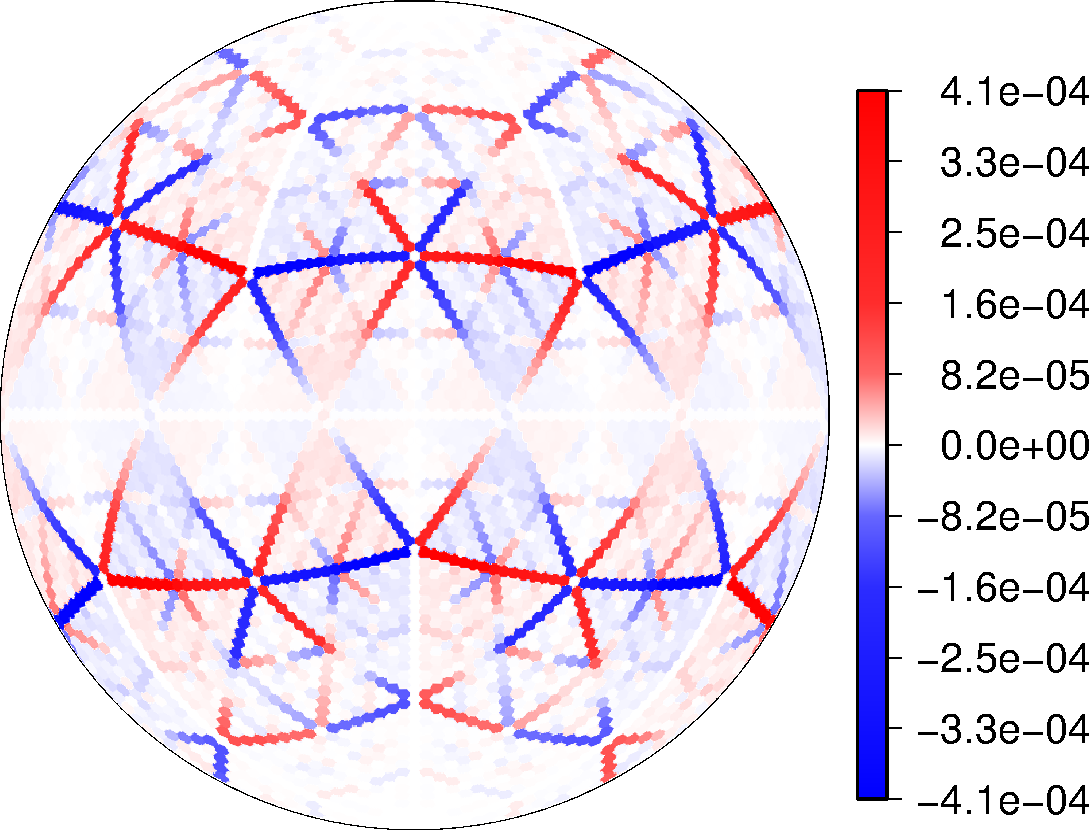
\includegraphics[scale=0.5]{divtest_f5_HC_error_icos_pol_nopt_5}

\section{Multigrid solver}

This part of the code was developed by Marline I. Silva in Sept 2014. It reads the parameter from par/multigrid.par and runs several tests for the multigrid solver. Select the following test case in par/mesh.par to run this program:\\
!  case(11)!Multigrid tests

This part of the code has not been thoroughly debug, and some tiding up may be necessary.


\section{Transport model}

The transport model is a Semi-Lagrangian as described in \cite{Peixoto2013b} and \cite{Peixoto2014}. You can run several test cases editing par/trans.par and selecting in par/mesh.par the following cases:\\
!  case(9) !Passive advection simulation\\
!  case(10)!Transport flow simulation\\

There is GMT script to create animations in gmt/anim.sh - please refer to it on usage.

\section{Shallow Water Model}

The shallow water model is a finite volume method with some methods implemented. The main module is swm.f90. First it has the TRSK method of \cite{Thuburn2009} and \cite{Ringler2010}, but also the modified scheme proposed in \cite{Peixoto2015}. Edit par/swm.par to configure the shallow water model. 

!Test Cases implemented\\
2 : Steady State Will92\\
5 : Flow over mountain Will92\\
6 : Rossby-Haurwitz Will92 \\
11 : Linearized equations - for mode calculation - fsphere\\
12 : Linearized equations - for mode calculation - f variable\\
21 : Galewski et al Barotropically unstable jet with perturbation\\
22 : Galewski et al Barotropically unstable jet without perturbation\\
32 : Hollingsworth instability with tc2\\
33 : Hollingsworth instability with constant h and non rotating frame  \\
42 : Rotated Steady state localised test on f-sphere\\
51 : Flow over mountain Will92 smooth mountain (Gaussian)\\

Some test cases rely on reference solutions to calculate errors. These solutions, if wanted, need to be pre-computed from the reference folder (ref/) with the ENDGame shallow water model - there is special documentation file in that folder to help.

To set up the new modified scheme proposed in \cite{Peixoto2015}, set in swm.par the following parameters:
\begin{verse}
!Scalar/vector location (HC or HTC) \\
HC \\
!Cell vec reconstruction method (Kenergy) / Gassmann parameter (if gass set) \\
perhx 0.75 \\
!Coriolis vec reconstruction method \\
pered \\
!Scalar interpolations \\
bary \\
!Gradient discrete method \\
trsk \\
\end{verse}
You also should set the HR95 grids to be read in par/mesh.par - the grid generator is not able to generate these with the same properties as in \cite{Heikes1995a}, so the .xyz grid nodes must be provided.

For TRSK, use
\begin{verse}
!Scalar/vector location (HC or HTC) \\
HTC \\
!Cell vec reconstruction method (Kenergy) / Gassmann parameter (if gass set) \\
trsk 0.75 \\
!Coriolis vec reconstruction method \\
trsk \\
!Scalar interpolations \\
trsk \\
!Gradient discrete method \\
trsk \\
\end{verse}

You can get the preprint of \cite{Peixoto2015} in \url{www.ime.usp.br/~pedrosp}, but I do appologise that some of the notation is different in the paper and code. Please contact me if you wish to have pre-calculated HR95 optimized grids.


\bibliographystyle{plainnat}% citação bibliográfica alpha
\bibliography{bibliography}  % associado ao arquivo: 'bibliografia.bib'



\end{document}
